\documentclass[a4paper]{article}

\usepackage{pgfplots}
\usetikzlibrary{patterns}

\pgfplotsset{compat=1.9}

\begin{document}

%\tracingcommands=2\tracingmacros=2
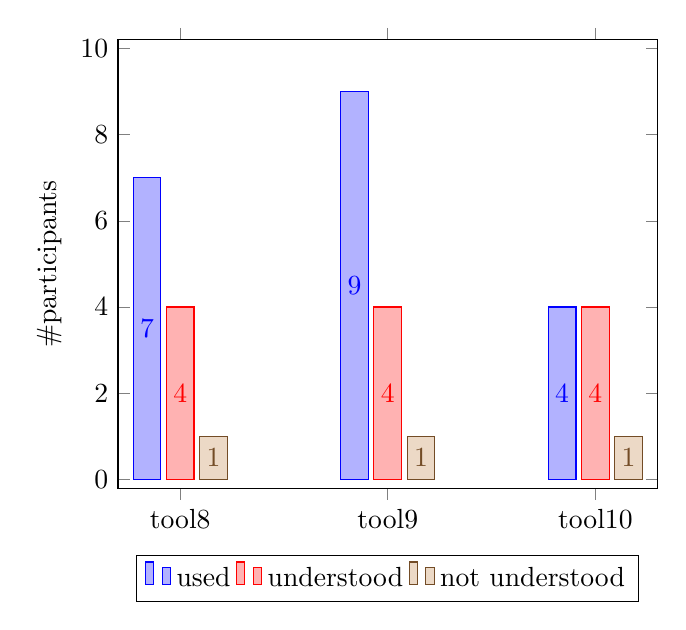
\begin{tikzpicture}
\begin{axis}[
    ybar,
    enlargelimits=0.15,
    legend style={at={(0.5,-0.15)},
      anchor=north,legend columns=-1},
    ylabel={\#participants},
    symbolic x coords={tool8,tool9,tool10},
    xtick=data,
	nodes near coords ybar stacked configuration,
    nodes near coords,
    ]
\addplot coordinates {(tool8,7) (tool9,9) (tool10,4)};
\addplot coordinates {(tool8,4) (tool9,4) (tool10,4)};
\addplot coordinates {(tool8,1) (tool9,1) (tool10,1)};
\legend{used,understood,not understood}
\end{axis}
\end{tikzpicture}


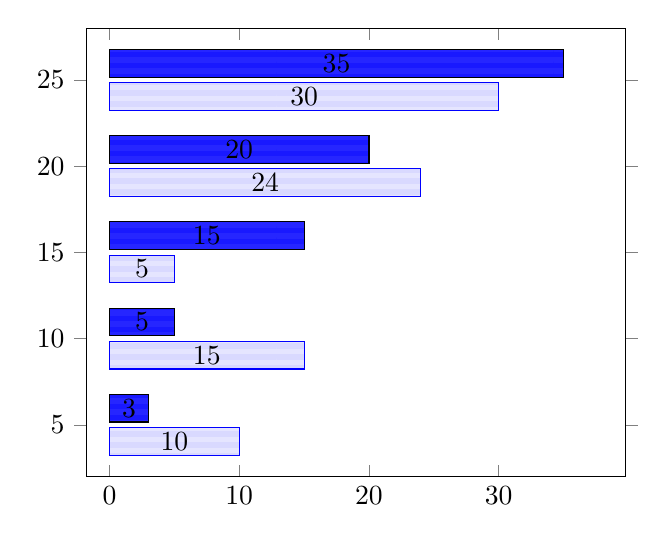
\begin{tikzpicture}
\begin{axis}[xbar,enlargelimits=0.15,
	nodes near coords xbar stacked configuration,
    nodes near coords,
]
\addplot
[draw=blue,pattern=horizontal lines light blue]
coordinates
    {(10,5) (15,10) (5,15) (24,20) (30,25)};
\addplot
[draw=black,pattern=horizontal lines dark blue]
coordinates
    {(3,5) (5,10) (15,15) (20,20) (35,25)};
\end{axis}
\end{tikzpicture}


\end{document}

